\chapter{Conclusion}
\label{chp:conclusions}
This desktop study was motivated by the consideration of sea level from within the Australian Bureau of Meteorology, and certain conceptual problems identified behind operational developments.
Exploration of the intersection of conventional tide prediction and operational mesoscale ocean forecasts within the agency has highlighted nuanced issues of representation, system compatibility and user expectation that are relevant to the strategic direction towards ``seamless'' services.
As such, all evaluations treated here have intentionally not pursued higher fidelity coastal simulations, but instead directed attention to some less-studied aspects of evaluating and exploiting predictability with established operational systems.   

As a thesis with publication, much of the body of this document has been published as, or is in preparation for peer-reviewed academic papers.
%------------------------
\section{Findings summary}
In answer to the research questions posed in chapter \ref{chp:introduction},  the findings of this thesis are summarised as follows:\\

Firstly, it was demonstrated that incompatible definitions of ocean ``tide'' are in parallel operational use.
Whereas downscaling for coastal sea level forecasts is clearly a productive approach, mesoscale ocean forecasts can immediately and directly provide significant but qualified forecast value for coastal sea level.
The fact that nominally tidal signals are present in mesoscale non-tidal ocean simulations means that care is required to avoid misinterpretation.

An aggregation approach that combines existing heterogeneous data but accounts for double-counting provides an important skill benchmark for future sea level forecast system development.
The point-based bias correction characteristics from these aggregated forecasts indicate that coastally contiguous extensions to model aggregation may be feasible.


In the operational context of combining and upgrading forecast models, it was shown that the coastal propagation characteristics of candidate forecast systems can be usefully evaluated and compared in a grid-independent waveguide projection.
Such a coastal waveguide projection also offers a means to direct forecaster attention to signals of special relevance along the Australian mainland coast.

Finally, it was argued that conventional harmonic tide predictions are not redundant, despite the ongoing advances in hydrodynamic simulation,  but that operational tide services require appropriate product differentiation to compliment modern applications and facilitate future refinement.
     % <<-- external file

%------------------------
\section{Heterogeneous simulations and seamless services}
The original coinage of "seamless" prediction in the context of climate projections has evolved to now encompass the more general goal of prediction across time and length scales \citep{10.1127/metz/2020/1048}.
Indeed the development of more seamless services is a strategic goal of the Australian Bureau of Meteorology \citep{BOM2020}.
\citep{10.1175/bams-89-4-459} illustrated the concept with a schematic chain of scales reaching from the small and fast out to the large and slow.
The present focus on sea level forecasting allows for a twist on the chain image to highlight the unusual place in which the LTI tidal admittance approach can be located relative to the geophysical fluid suite of simulations.
Figure \ref{fig:forecastScalesChain} schematically shows that tide prediction in general can provide very long horizon prognoses of short time scale fluctuations in sea level; of course subject to many caveats.
%------------------------------
\begin{figure}[h]\centering
        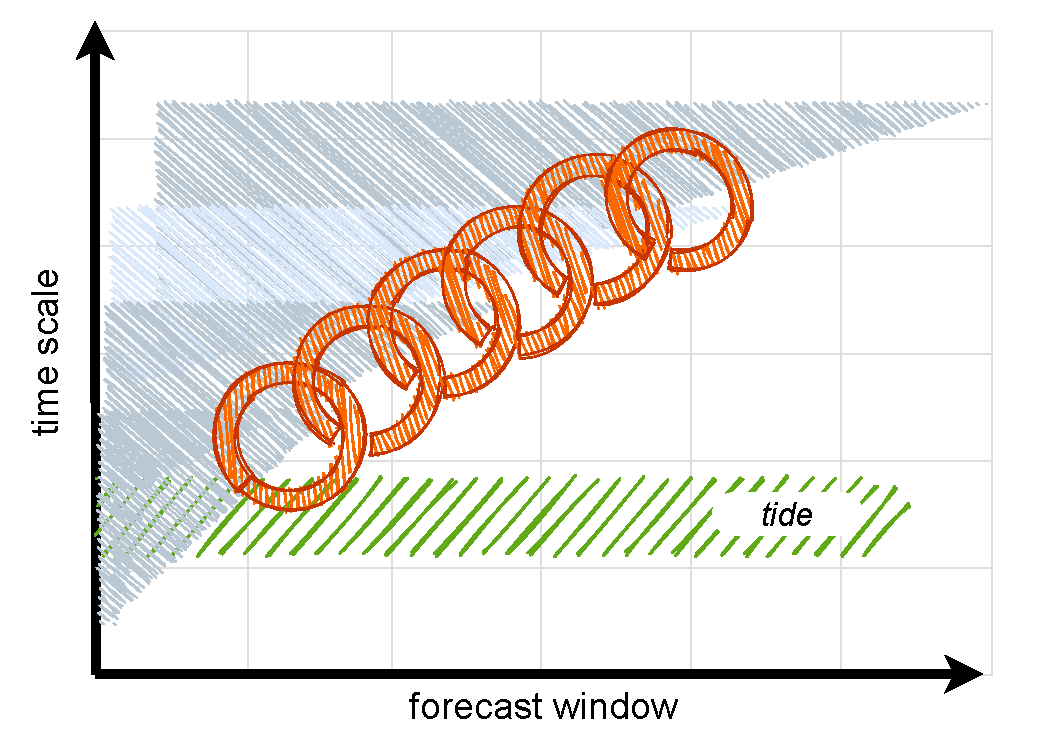
\includegraphics[width=\figwidthFull]{figures/diagrams/scales_with_chain.pdf} 
        \caption{Schematic place of tide prediction in model scales using chain image.}
                {Tide prediction can sit awkwardly with the seamless chain-of-scales analogy and highlights an ongoing role for forecast method heterogeneity; following Figure \ref{fig:forecastScalesAll} and \citep{10.1175/bams-89-4-459}}
        \label{fig:forecastScalesChain}
\end{figure}
%------------------------------
The intention behind this imagery is to emphasise that multi-scale prediction need not be shoe-horned into the tidy cascade of a single consistent earth system simulation framework.
Although a consistent framework and a single simulation code-base is very attractive on multiple fronts  \footnote{\url{https://research.csiro.au/access/what/}}, consideration of the status of sea level and tide prediction provides at least one case in which some sort of exception is sure to be required based on the unique value offered by particular mechanisms and legacy products.  

Operational forecasting today, when viewed holistically, is based on a suite of systems that are not cleanly compatible.
The prognostic potential of Australian Bureau of Meteorology has arguably not been fully realised to some degree as a result of system heterogeneity.  Consider how the forecast information published variously as maps of non-tidal sea level anomaly, storm surge warnings and tide-table products cannot self-evidently be synthesized and directly interpreted in relation to observable sea level.
Whilst progress towards ever more concrete and consistent earth simulations will continue apace, there is sure to be an ongoing operational requirement to handle inhomogeneity and system transitions in manner that actually provides useful forecast value. Moreover, realising that value will require ``\textit{closer and wider cooperation between the scientific community, stakeholders, policy- and decision-makers to ensure that sea level products are accessible and are used correctly and appropriately...}'' in line with the final recommendation of \citet{10.1175/bams-89-4-459}. 

%------------------------
\section{Next steps}
The will be ongoing opportunities to improve sea level forecast services as the operational suite of simulation systems improve, but any innovation will necessarily be interpreted by users against the background of conventional tide predictions.

Whilst this body of work intentionally restricted focus to the Australian setting, some of the higher level  characterisations will be translatable to other shores, especially the basic conceptual overlap between aspects of conventional tide prediction and hydrodynamic simulation.
The federated jurisdiction combined with the vast expanse of the Australian coast tips the balance of operational challenges towards delivering a more universal, as opposed to highly targeted, approach to forecasting.   As a jurisdictional contrast is available in the case of South Korea, where a dense network of weather and marine observations are maintained under the same auspices as the forecasting agency (eg   
\citep{Suh:2015fy}).
The vast Australian coast also raises the significance of large scale coastal propagation, and moreover highlights the problem of observation sparsity.


There remains a primary role for tide gauge observations to underpin sea level forecasting across the board.
Expansion of the observation capabilities to new platforms, be it video \citep{10.1175/jtech-d-18-0203.1} or wide swath altimetry, will not side-step the ongoing role for tide gauges.
\citep{Keysers:we} emphasised the need for not only a denser network of observations around the Australian coast, but a national repository and ongoing curation of sea level observations and survey connections to support the needs of precision positioning.   
That call is effectively mirrored for forecasting applications in the recommendations of \citep{10.1175/bams-89-4-459}.
As yet, there is no such Australian coordination; at least not in the sense of seamlessly serving real-time and survey applications.
There is an obvious opportunity to better align the capabilities of the conventional tide service, operational forecasting and spatial survey to maintain a foundational public resource.  Whilst small steps have been taken in that direction by the Intergovernmental Committee on Surveying and Mapping \footnote{\url{https://www.icsm.gov.au/}}, progress would be a great enabler for improved sea level forecast services.





Finally, consideration of how tides and sea level fit within the operational setting of the Bureau of Meteorology corroborates the need for a concept of forecasting services that juxtaposes the chain-of-scales model; namely the so-called `micro-service' architecture \citep{BCG2020}.   This architecture is not in opposition to the seamless ideal, but is perhaps best thought of as orthogonal.  
Quite apart from the vision for an all-encompassing multi-scale earth system simulation, the extraction of value from forecasts more generally appears to be on a fast trajectory towards the downstream combination of heterogeneous inputs for bespoke decision support applications.  
Ensuring that forecast outputs of all sorts are machine-readable, discoverable and well-characterised will facilitate the development of improved sea level applications both within and external to the operational agency itself.    

%is increasingly relevant to government services and is embodied by programs such as  \url{api.gov.au}) and the International Hydrographic Organisations  navigation-focused exchange specifications (\url{http://s100.iho.int}).



